\section{Auxilary Construction}\label{sec:auxiliaryConstruction}
Given an instance $\Phi$ of P3SAT with $n$ variables and $m$ clauses and its associated graph $A(\Phi)$, we construct a simply connected polygonal linkage $(\PP,H)$, of polynomial size in $n$ and $m$, such that $\Phi$ is satisfiable if and only if $(\PP,H)$ admits a realization with fixed orientation. 

We construct a polygonal linkage  in two main steps: first, we construct an auxiliary structure where some of the polygons have fixed position in the plane (called \emph{obstacles}), while other polygons are flexible, and each flexible polygon is hinged to an obstacle. 
Second, we modify the auxiliary construction into a polygonal linkage by allowing the obstacles to move freely, and by adding new polygons and hinges as well as an exterior \emph{frame} that holds the obstacle polygons in place.
All polygons in our constructions are regular hexagons or long and skinny rhombi because these are the polygons that we can ``simulate'' with disk arrangements in Section~\ref{sec:disk}.

Let $\Phi$ be a Boolean formula of P3SAT with variables $x_1,\ldots , x_n$ and clauses $C_1,\ldots ,C_m$, where $A(\Phi)$ is the associated planar graph and $\tilde{A}\lr{\Phi}$ be corresponding honeycomb graph.
We continue to modify $\tilde{A}\lr{\Phi}$ to form the auxilary construction.   
For each hexagon in $\tilde{A}\lr{\Phi}$, we scale the hexagons in the following way: first we fix the center of the hexagon and then scale (shrink) the hexagon; the hexagons in the honeycomb no longer touch each other and form corridors and junctions between the hexagons. 
Formally, let a \textit{corridor} be a channel between two adjacent hexagons and a \textit{junction} be a region where three corridors meet.
We then finally re-scale this form of the honeycomb such that the side length of the hexagons are determined by polynomial of variable $n$ and $m$, $N(n,m)$, while preserving the corridors formed from the first scaling.\newline

\begin{minipage}{\linewidth}
\begin{center}
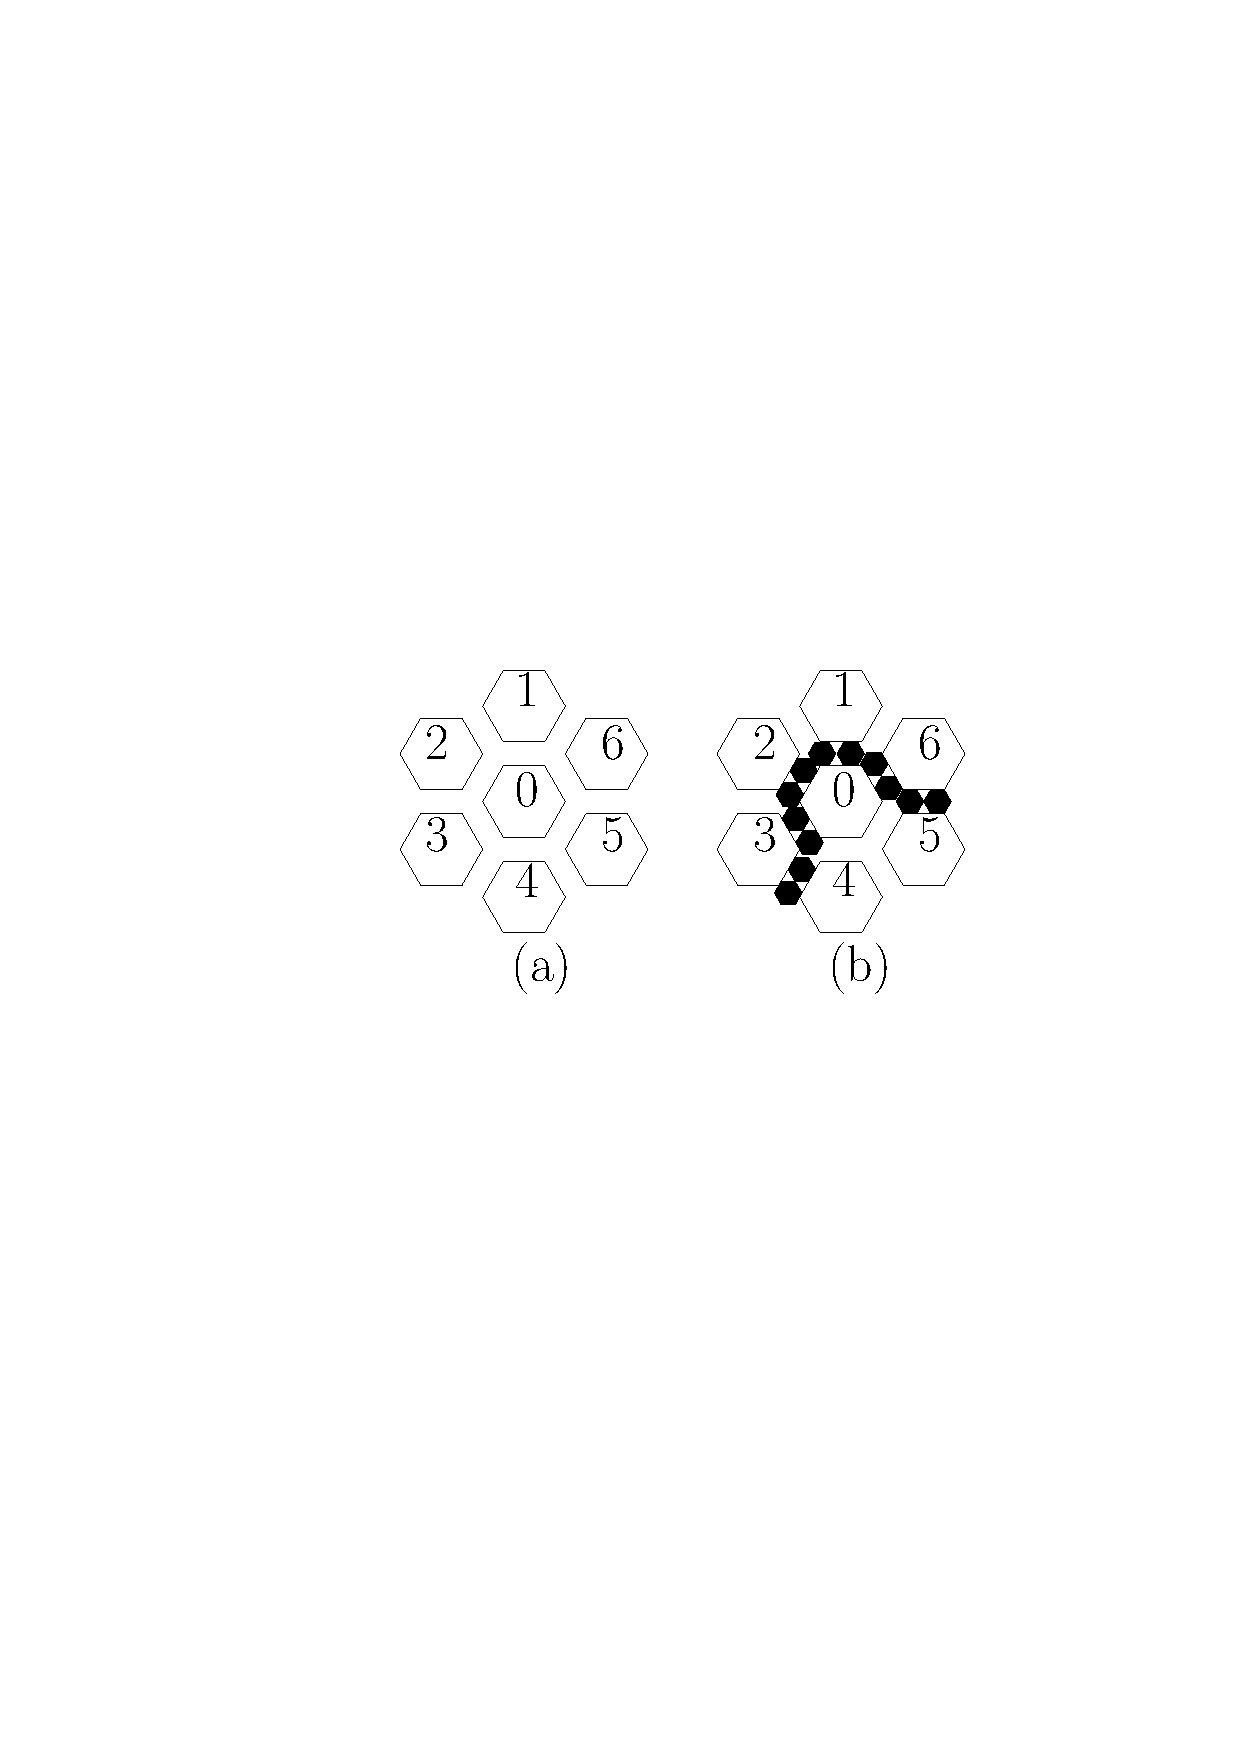
\includegraphics[scale=.66]{graphics/FlexibleHexagons.pdf}
\captionof{figure}{
(a) A region of the honeycomb shown with scaling. The corridors and junctions formed from the first scaling is preserved after scaling the honeycomb grid to where the side lengths of the hexagon are $N(n,m)$.
(b) The same region in (a) containing flexible hexagons.
}\label{fig:HoneycombFlixible.pdf}
\end{center}
%\end{figure}
\end{minipage}

Let the hexagons of Figure \ref{fig:HoneycombFlixible.pdf}(a) be obstacle hexagons that are fixed at their centers.
In Figure \ref{fig:HoneycombFlixible.pdf}(b), we have smaller hexagons within some corridors and junctions.
These hexagons are flexible hexagons.
For each edge in $\tilde{A}(\Phi)$, we will replace that edge with flexible hexagons.
Flexible hexagons are hinged at the vertex closest to origin and the side of the corridor (See Figure \ref{fig:variable}).
Let $t=2N^3+1$ be the number of flexible hexagons in a corridor (see Figure \ref{fig:variable}). 
Scale the honeycomb such that the obstacle hexagons become regular hexagons of side length $(5t-1)/2+\sqrt{3}$, and then scale each obstacle hexagon independently from its center to a hexagon of side length $(5t-1)/2$ (see Figure \ref{fig:honeycomb}). 
%Let $\Phi$ be a Boolean formula in 3-CNF with variables $x_1,\ldots , x_n$ and clauses $C_1,\ldots ,C_m$, and let $A(\Phi)$ be the associated planar graph.
%We modify $A(\Phi)$ to obtain a plane graph $\tilde{A}(\Phi)$ of maximum degree 3 as follows: replace each \emph{variable} vertex $v$ by a cycle whose length equals the degree of $v$, and distribute the edges incident to $v$ among the vertices of the cycle.
%Embed $\tilde{A}(\Phi)$ into the section of a hexagonal tiling (e.g. see Figure \ref{fig:HoneyCombAssociatedGraphSmall} and Figure \ref{fig:assoc}, right), contained in a regular hexagon of side length $N$, where $N$ is a polynomial of $n$ and $m$~\cite{BK+98}.
% \begin{figure}[htbp]
% 	\centering
% 	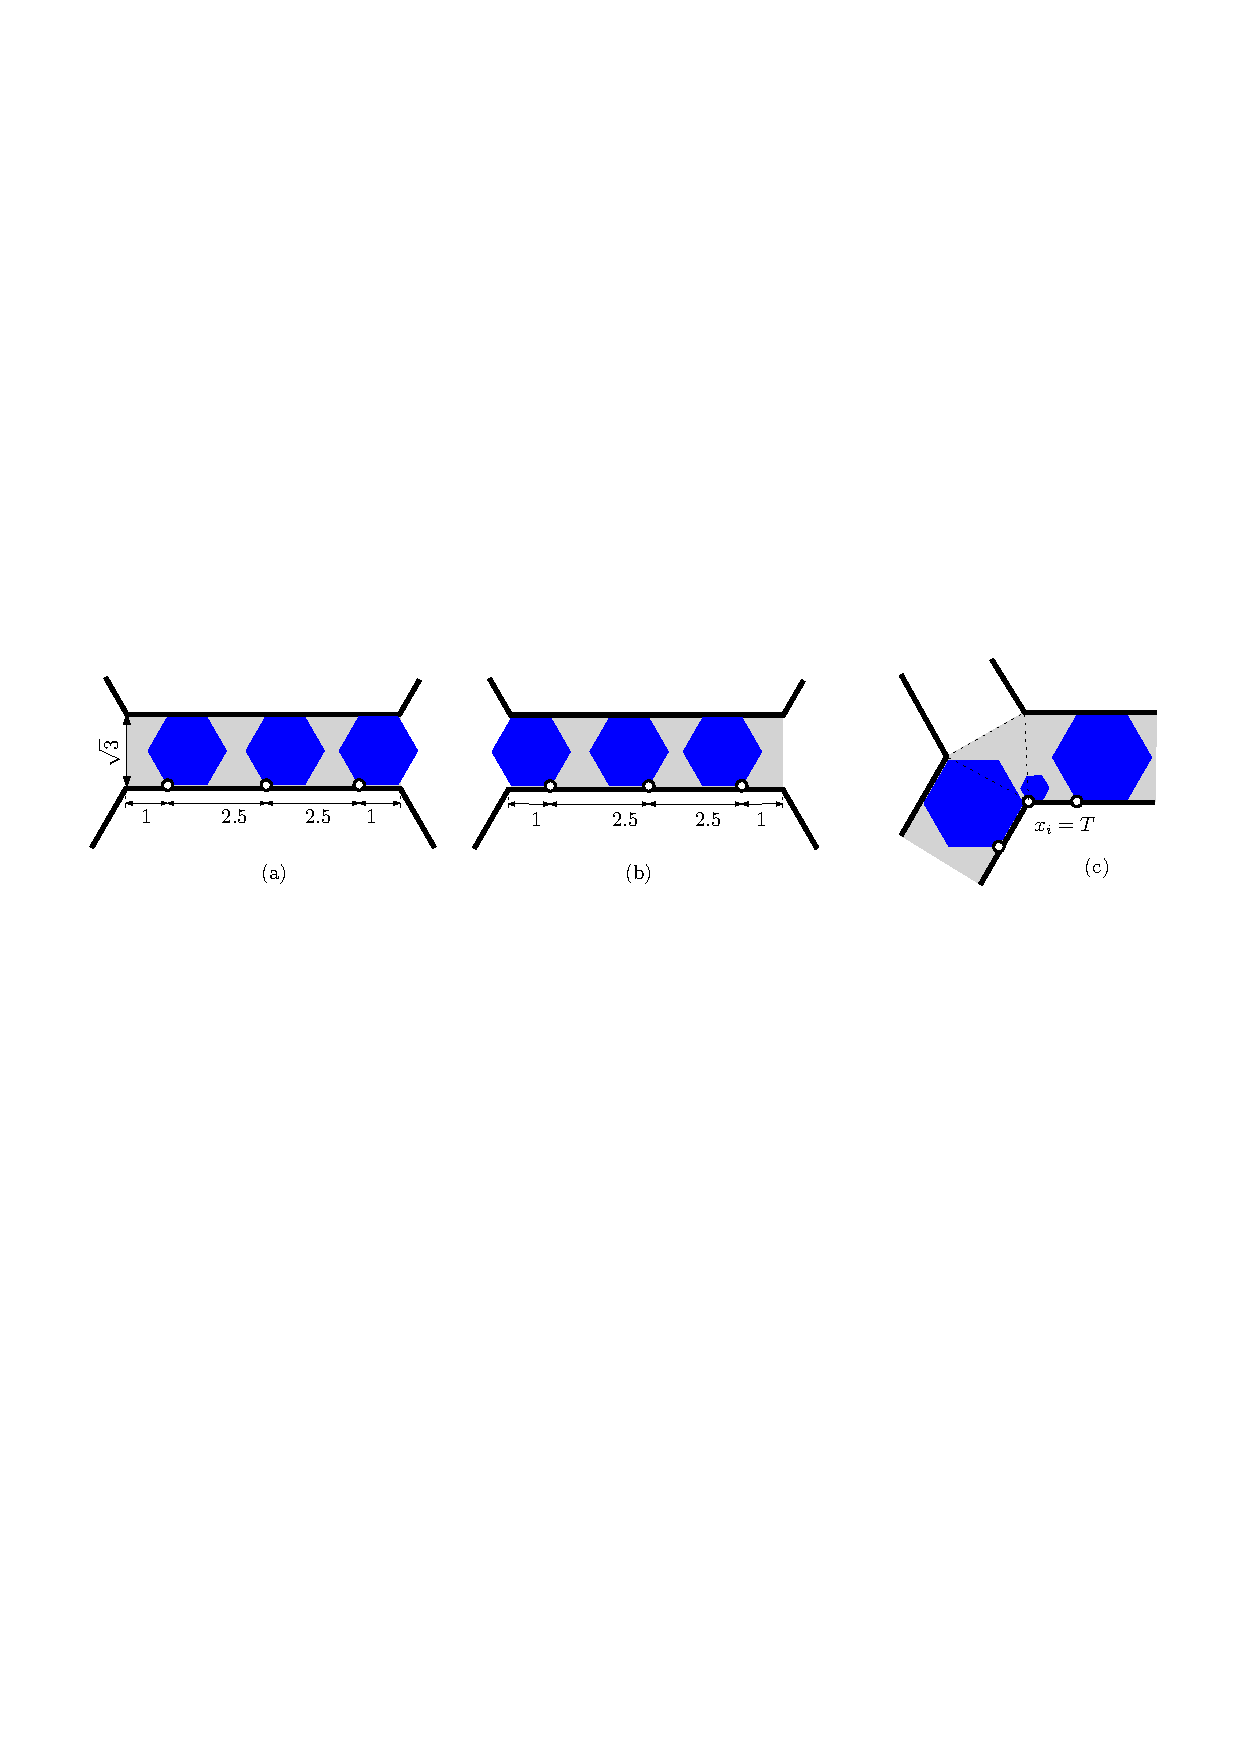
\includegraphics[width=0.9\columnwidth]{graphics/fig-variable-hex+}
% 	\caption{(a) A corridor when all unit hexagons are in state R.
% (b) A corridor where all unit hexagons are in state L.
% (c) A junction where a small hexagon between two corridors
%     ensures that at most one unit hexagon enters the junction from those corridors.}	
% \end{figure}

\begin{minipage}{\linewidth}
\begin{center}
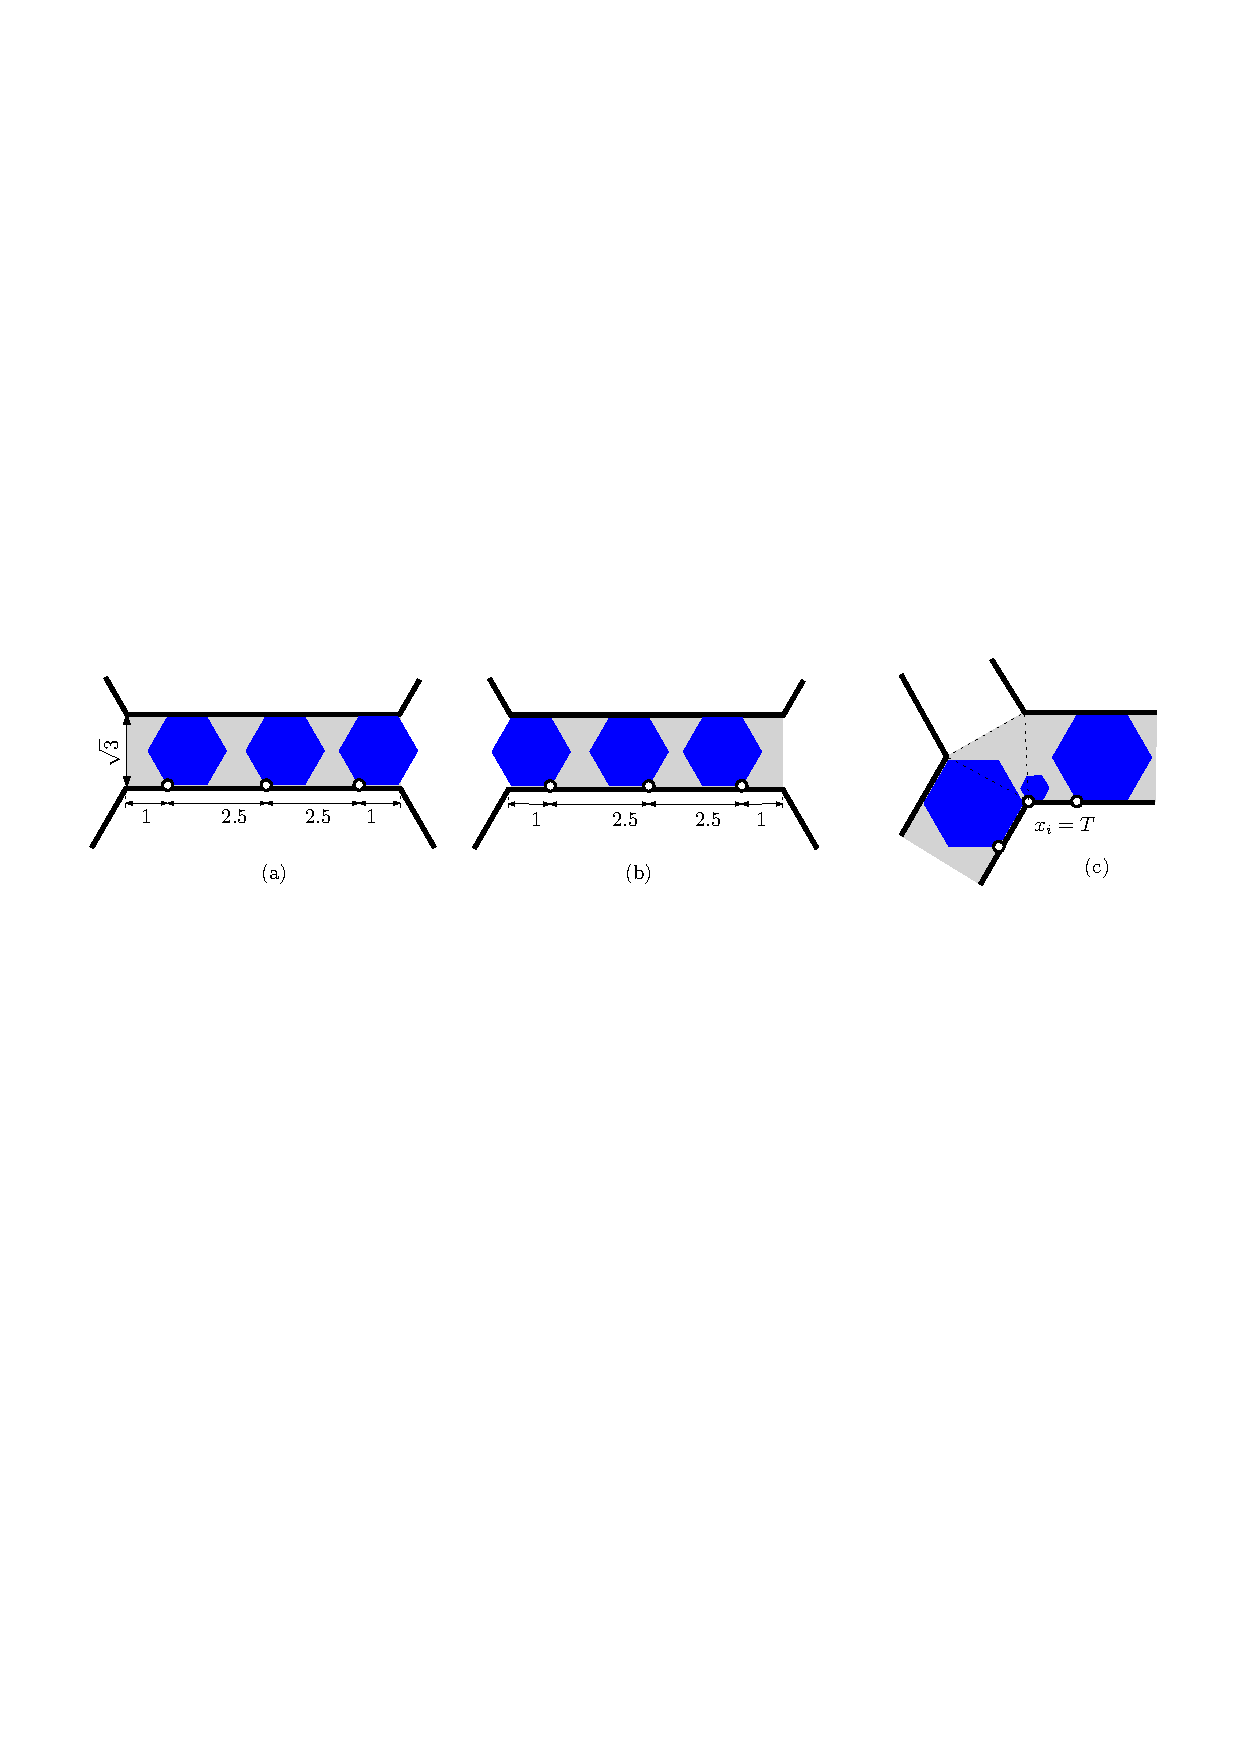
\includegraphics[width=0.9\columnwidth]{graphics/fig-variable-hex+}
\captionof{figure}{
(a) A corridor when all unit hexagons are in state R.
(b) A corridor where all unit hexagons are in state L.
(c) A junction where a small hexagon between two corridors
    ensures that at most one unit hexagon enters the junction from those corridors.}\label{fig:variable}
\end{center}
%\end{figure}
\end{minipage}

%These large hexagons are considered fixed obstacles in our auxiliary construction. 
Between two adjacent obstacle hexagons, there is a $\frac{5t-1}{2}\times \sqrt{3}$ rectanglar corridor.  %, which we call corridor. 
Three adjacent corridors meet at a regular triangle, which we call a \emph{junction}. 
We next describe variable, clause, and transmitter gadgets.

\begin{minipage}{\linewidth}
\begin{center}
\includegraphics[width=0.3\columnwidth]{graphics/honeycomb.pdf}
\captionof{figure}{The small honeycomb-like structure within the large hexagons depicts cells.}\label{fig:honeycomb}
\end{center}
%\end{figure}
\end{minipage}

The basic building block of both variable and transmitter gadgets consists of $t$ regular hexagons of side length 1 (\emph{unit hexagons}, for short) attached to a wall of a corridor such that the hinges divide the wall into $t+1$ intervals of length $(1,2.5,\ldots ,2.5,1)$ as shown in Fig.~\ref{fig:variable}(a-b) for $t=3$. 


% \begin{lem}
% If the leftmost hexagon is in state R, then all $t$ hexagons are in state R, and the rightmost hexagon enters the junction on the right of the corridor.
% \end{lem}
% \begin{proof}
% Suppose the left most hexagon, $h_1$, in a corridor is in state R and there are $t$ hexagons in the corridor. 
% $h_i$ for $i=2,\dots, t$ is in either state $R$ or $L$.
% $h_2$ must be in the state $R$ otherwise we result in a collision with 
% \end{proof}
Each junction is a regular triangle, adjacent to three corridors. 
In some of the junctions, we attach a small hexagon of side length $\frac{1}{3}$ to one or two corners of the junction (see Fig.~\ref{fig:variable}(c) and Fig.~\ref{fig:transmitter}). 
Importantly, we have the following observation:
\begin{observation}\label{obs:junction}
If a small hexagon is attached to a vertex between two corridors, then a unit hexagon can enter the junction from at most one of those corridors.
\end{observation}

\subsection{Variable Gadget}
The {\bf variable gadget} for variable $x_i$ is constructed as follows. 
Recall that variable $x_i$ corresponds to a cycle in the associated graph $\tilde{A}(\Phi)$, which has been embedded as a cycle in the hexagonal tiling, with corridors and junctions. 
In each junction along this cycle, attach a small hexagon in the common boundary of the two corridors in the cycle. 
Figure \ref{fig:VariableGadgetSmall.pdf} depicts a \textit{variable gadget} in the hexagonal grid.

\begin{minipage}{\linewidth}
\begin{center}
\includegraphics[width=0.45\columnwidth]{graphics/VariableGadgetSmall.pdf}
\captionof{figure}{This depicts a variable gadget with $x_1 = T$.  Carefully note that the flexible hexagons around $x_1$ are in the state $R$. Corridors adjacent to two obstacles of a variable in the honeycomb do not have $t$ flexible hexagons; these corridors simply have the flexible hexagons at the junctions.}\label{fig:VariableGadgetSmall.pdf}
\end{center}
%\end{figure}
\end{minipage}

Observation~\ref{obs:corridor} and the small hexagons ensure that the state of any unit hexagon along the cycle determines the state of all other unit hexagons in the cycle. 
This property defines the binary variable $x_i$: If $x_i=T$, then all unit hexagons in the top horizontal corridors are in state R; and if $x_i=F$, they are all in state L.
\begin{figure}[htbp]
	\centering
	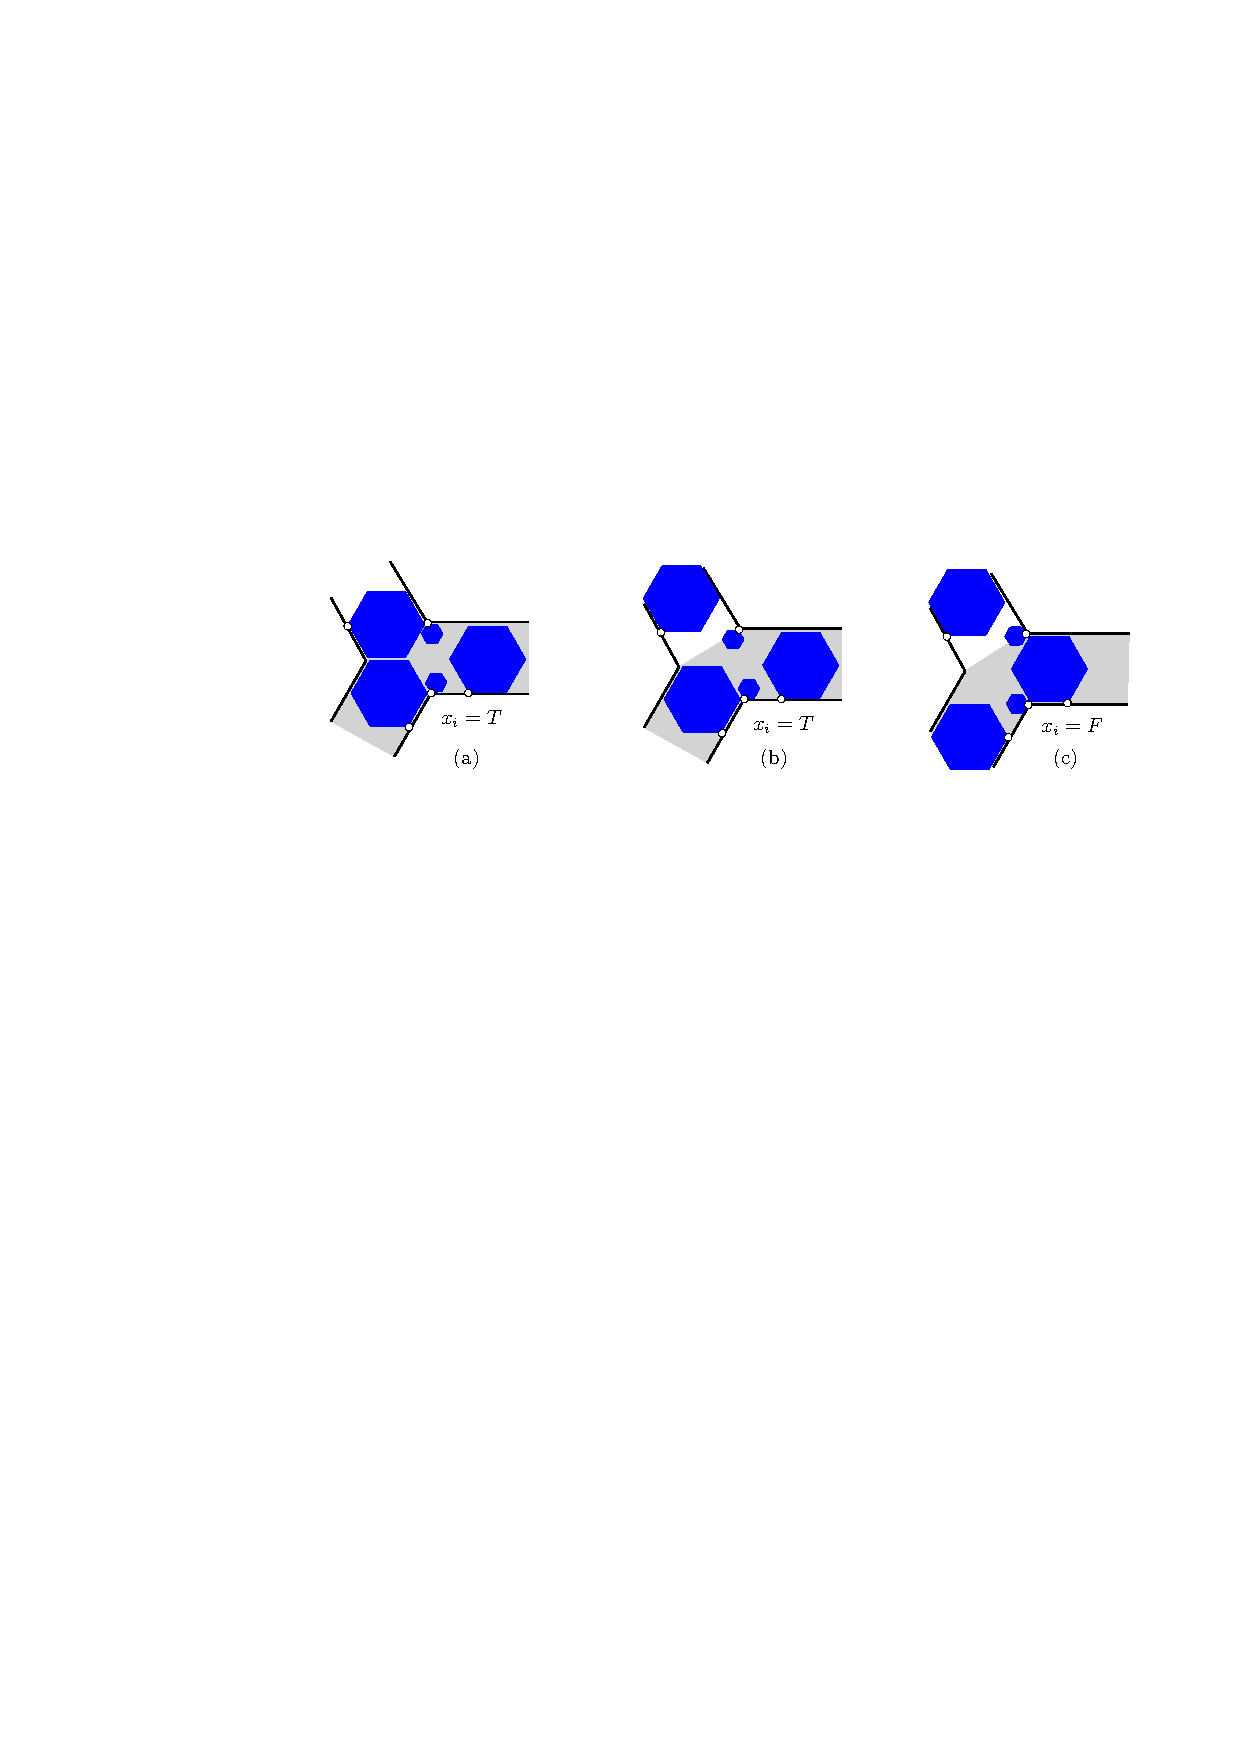
\includegraphics[width=0.7\columnwidth]{graphics/fig-transmitter-hex}
	\caption{The common junction of a variable gadget and a transmitter gadget.
(a) When $x_i=T$, a hexagon of the transmitter may enter the junction of the variable gadget.
(b) When $x_i=T$, the transmitter gadget has several possible realizations.
(c) When $x_i=F$, no hexagon from the transmitter enters a junction of the variable gadget.}
	\label{fig:transmitter}
\end{figure}
When a binary variable $x_i = T$, we will say that the variable in state $R$ and that the cycle of small hexagons around the variable gadget are in a ``clockwise direction''.
When a binary variable $x_i = F$, we will say that the variable is in state $L$ and that the cycle of small hexagons around the variable gadget are in a ``counter-clockwise direction''. 

\subsection{Clause Gadget}
Recall that a clause from a Boolean formula $\Phi$ in 3-CNF has three literals.  If $\Phi$ is a  'yes' instance, then at least one literal in every clause of $\Phi$ is true.  We construct the clause gadget to model this fact about Boolean formulas in 3-CNF.

The {\bf clause gadget} lies at a junction adjacent to three transmitter gadgets (see Fig.~\ref{fig:clause} and Section \ref{transmitterGadget}). 
At such a junction, we attach a unit line segment to an arbitrary vertex of the junction, and a small hexagon of side length $\frac{1}{3}$ to the other end of the segment. 
If unit hexagons enter the junction from all three corridors (i.e., all three literals are false), then there is no space left for the small hexagon. 

\begin{minipage}{\linewidth}
\begin{center}
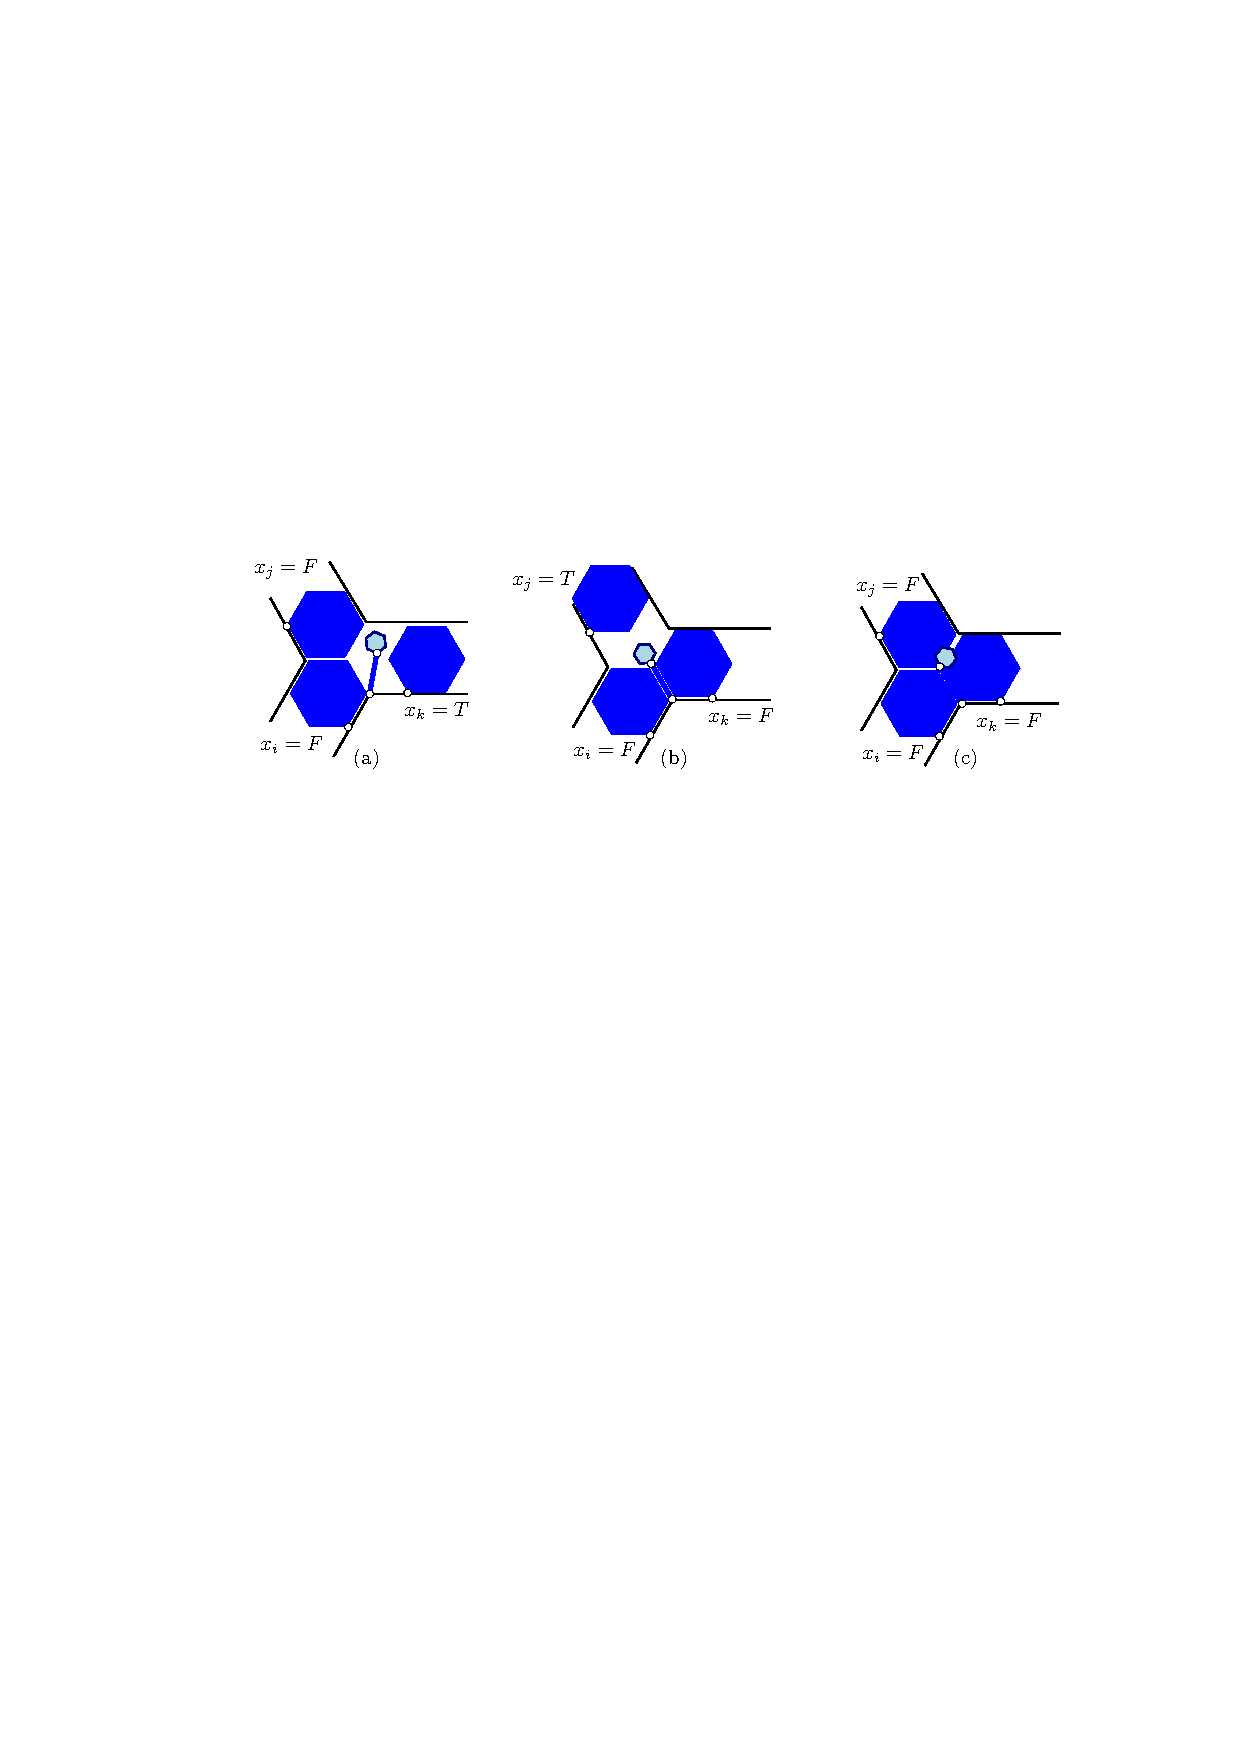
\includegraphics[width=0.7\columnwidth]{graphics/fig-clause-hex}
\captionof{figure}{(a-b) A clause gadget $(x_i\vee x_j\vee x_k)$ is
    realizable when at least one of the literals is {\sc True}.
    (c) The clause gadget cannot be realized when all three literals are {\sc False}.}\label{fig:clause}
\end{center}
%\end{figure}
\end{minipage}

But if at most two unit hexagons enter the junction (i.e., one of the literals is true), then the unit segment and the small hexagon are realizable.
\subsection{Transmitter Gadget}\label{transmitterGadget}
A {\bf transmitter gadget} is constructed for each edge $(x_i,C_j)$ of the graph $A(\Phi)$.
It connects a junction of the variable gadget $x_i$ with the junction representing the clause gadget $C_j$. 
The gadget consists of a path of corridors and junctions: at each interior junction, attach a small hexagon in the common boundary of the two corridors in the path (similarly to the variable gadget).

\begin{minipage}{\linewidth}
\begin{center}
\includegraphics[width=0.45\columnwidth]{graphics/TransmitterGadgetSmall.pdf}
\captionof{figure}{This depicts a transmitter gadget connected with the variable gadget shown in Figure \ref{fig:VariableGadgetSmall.pdf}.  }\label{fig:TransmitterGadgetSmall.pdf}
\end{center}
%\end{figure}
\end{minipage} 

At the common junction with the variable gadget $x_i$, we attach one additional small hexagon to one of the vertices (refer to Fig.~\ref{fig:transmitter}). 
If the literal $x_i$ (resp., $\overline{x}_i$) appears in $C_j$, then we attach a small hexagon to the corner of this junction such that if $x_i=F$ (resp., $\overline{x}_i=F)$, then the unit hexagon of the transmitter gadget cannot enter this junction. 
The junction placement of a transmitter gadget depends upon the variable's state, $R$ or $L$.
When the variable is false (i.e. state $L$), the tranmitter is place on a right-most junction above a variable gadget's obstacle hexagon or a left-most junction below a varaiable gadget's obstacle hexagon.
Similarly, when the variable is true (i.e. state $R$), the tranmitter is place on a left-most junction above a variable gadget's obstacle hexagon or a right-most junction below a varaiable gadget's obstacle hexagon.
When $x_i = F$ , no hexagon from the transmitter enters a junction of the variable gadget.
This ensures that false literals are always correctly transmitted to the clause junctions (and true literals can always transmit correctly).

A variable gadget for vertex $v$ in the associated graph of a P3SAT Boolean formula encompasses at least $2 \cdot \deg (v)$ consecutive obstacle hexagons. 
The arrangement of the consecutive obstacle hexagons are in staggered fashion where there are at least $\deg (v)$ obstacle hexagons in the upper portion of the staggering arrangement and at least $\deg (v)$ obstacle hexagons in the lower portion of the staggering arrangement.
To construct all transmitter gadgets corresponding to the edges of an associated graph of a P3SAT instance, there must be at least $\deg (v)$ left-most junctions and $\deg (v)$ right-most junctions in both the upper portion of the variable gadget and the lower portion of the variable gadget.
Suppose the variable $v$ exists only in clauses that lie above the variable gadget.  
The construction of the variable gadget allows for $\deg (v)$ placements of transmitters on either the left or right side of the upper obstacle hexagons accordingly.
Similarly, suppose the variable $v$ exists only in clauses that lie above the variable gadget.  
The construction of the variable gadget allows for $\deg (v)$ placements of transmitters on either the left or right side of the lower obstacle hexagons accordingly.
Each obstacle hexagon has a left and right junction to admit a transmitter gadget to connect to.

\begin{figure}[!htb]
    \centering
    \begin{minipage}{.45\textwidth}
        \centering
        \includegraphics[scale=.33]{graphics/VariableTrueTransmitterClause.pdf}
        \caption{Variable $x_i$ with state $R$ transmitting the non-negated literal $x_i$ into clause $C_j$.}
        \label{fig:VariableTrueTransmitterClause.pdf}
    \end{minipage}%
    \begin{minipage}{0.45\textwidth}
        \centering
        \includegraphics[scale=.33]{graphics/TrueVariableNegatedLiteralTransmitter.pdf}
        \caption{Variable $x_i$ with state $R$ transmitting the negated literal $\lnot x_i$ into clause $C_j$.}
        \label{fig:TrueVariableNegatedLiteralTransmitter.pdf}
    \end{minipage}
\end{figure}

\begin{figure}[!htb]
    \centering
    \begin{minipage}{.45\textwidth}
        \centering
        \includegraphics[scale=.5]{graphics/FalseVariableNonNegatedLiteralTransmitter.pdf}
        \caption{Variable $x_i$ with state $L$ transmitting the non-negated literal $x_i$ into clause $C_j$.}
        \label{fig:FalseVariableNonNegatedLiteralTransmitter.pdf}
    \end{minipage}%
    \begin{minipage}{0.45\textwidth}
        \centering
        \includegraphics[scale=.35]{graphics/VariableFalseTransmitterClause.pdf}
        \caption{Variable $x_i$ with state $L$ transmitting the negated literal $\lnot x_i$ into clause $C_j$.}
        \label{fig:VariableFalseTransmitterClause.pdf}
    \end{minipage}
\end{figure}
% \begin{figure}[htbp]
% 	\centering
% 	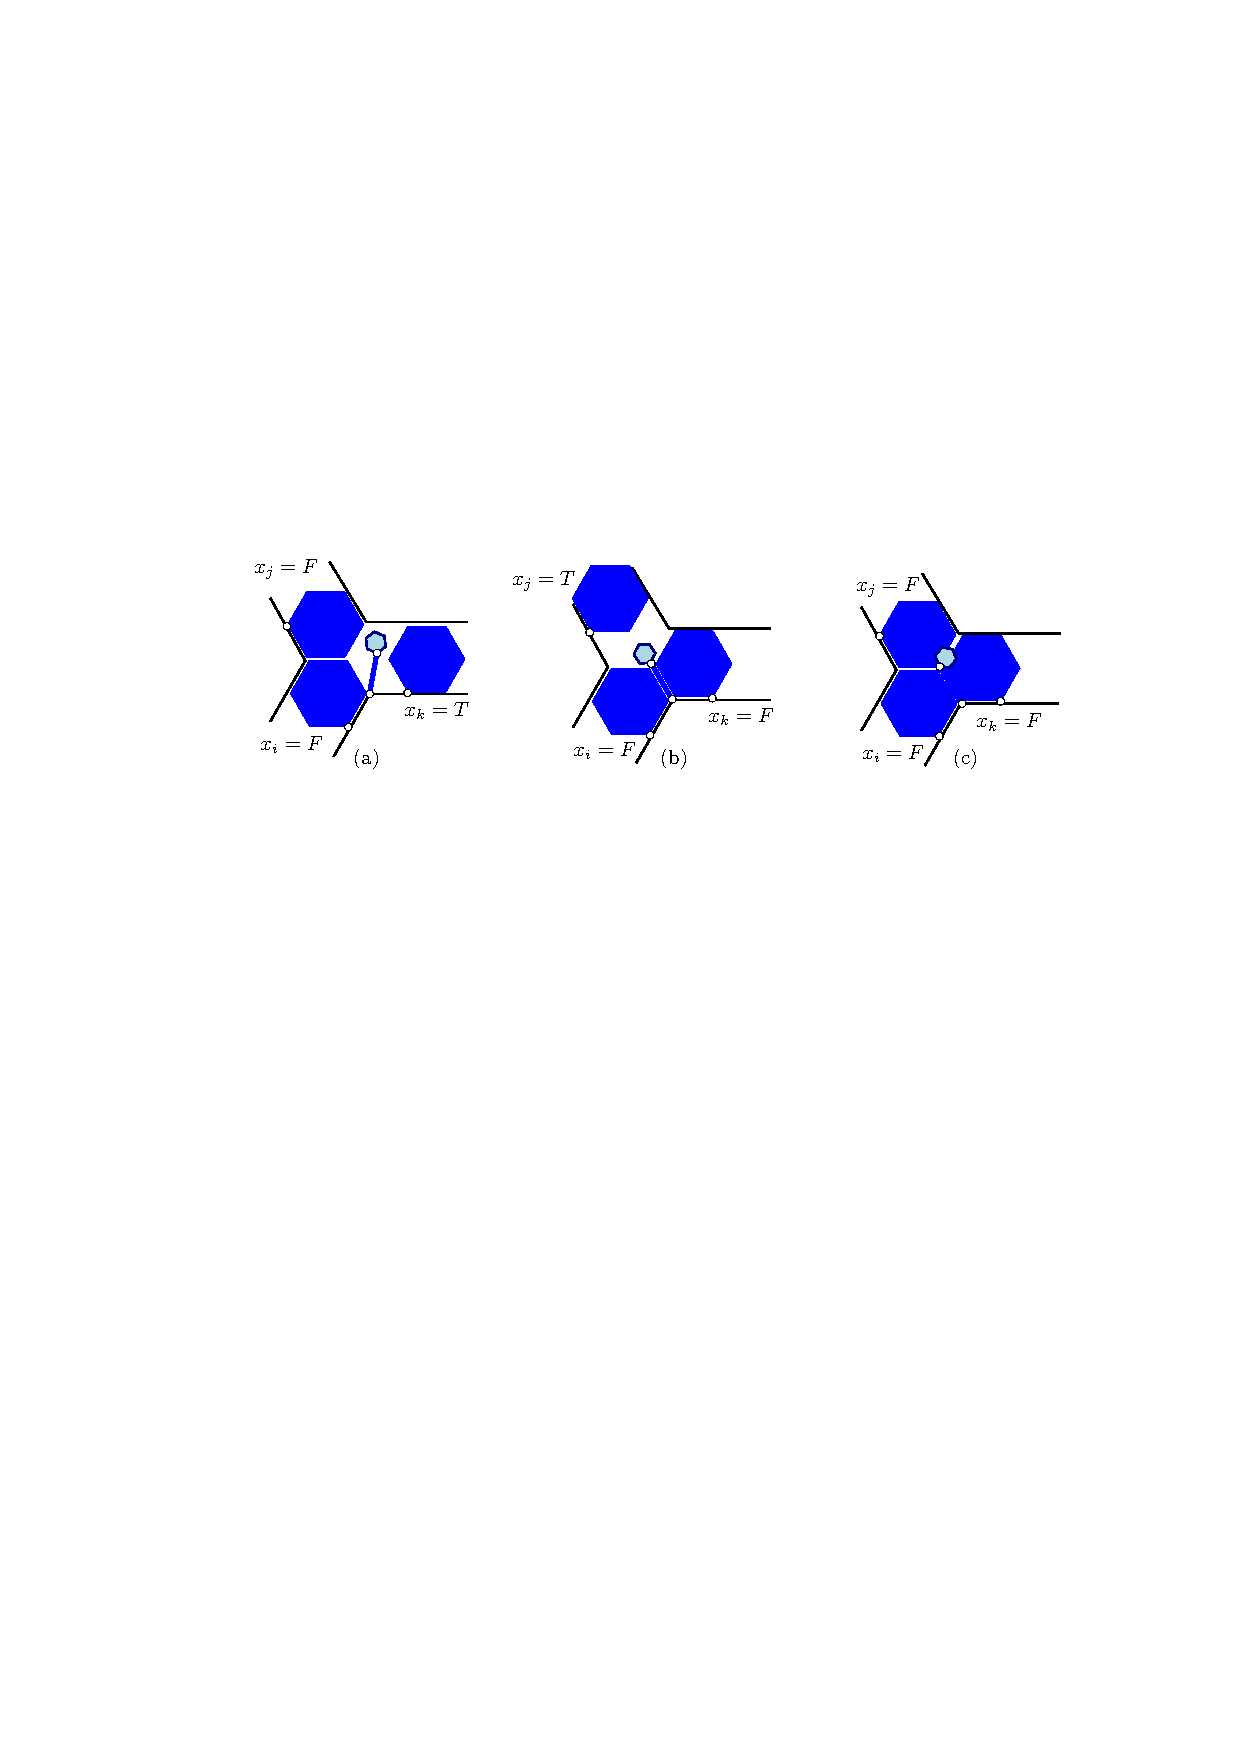
\includegraphics[width=0.7\columnwidth]{graphics/fig-clause-hex}
% 	\caption{(a-b) A clause gadget $(x_i\vee x_j\vee x_k)$ is
%     realizable when at least one of the literals is {\sc True}.
%     (c) The clause gadget cannot be realized when all three literals are {\sc False}.}
% 	\label{fig:clause}
% \end{figure}





% \begin{thm}\label{thm:chp2-HingedPolygons-1}
%  Given an instance of a $NAE3SAT$,  it is a ``yes'' instance if and only if the 
% corresponding polygonal linkage logic engine has a collision-free configuration.  
% \end{thm}
% \begin{proof}
% Suppose we have an instance of a $NAE3SAT$ that is a ``yes'' instance. This implies that there is a 
% truth assignment such that each clause contains a true and a false literal. Now consider the polygonal linkage logic 
% engine corresponding to this instance. We now 
% show that it has a collision free configuration.

% For variables that are true, configure the armatures such that the flags corresponding to the 
% non-negated literals reside above the 
% shaft and the flags that correspond to the negated literals reside below this shaft.  For variables 
% that are false, configure the 
% armatures in the opposite orientation.  Each clause corresponds to a pair of rows in 
% the polygonal linkage logic engine, one row for non-negated literals and one for negated literals.  Because the 
% $NAE3SAT$ is a yes instance, every row contains at least one unflagged armature.  
% By Lemma \ref{lem:logicEngine1}, every row  has a collision-free configuration.

% Suppose we have an instance of a $NAE3SAT$ such that the corresponding polygonal linkage logic engine has a 
% collision-free configuration. By Lemma \ref{lem:logicEngine1} every row at least one unflagged 
% armature.  The $k^{th}$ clause is represented by the $k^{th}$ rows above and below the shaft. If the 
% literal $x_j$ is found in clause $C_k$, then the armature is unflagged in that row. If the literal 
% $\bar{x}_j$ is found in clause $C_k$, then $\bar{l}_{j,k}$ is unflagged.  All flags 
% corresponding to negated literals reside below the shaft and flags corresponding to non-negated 
% literals reside above the shaft.  All together we have that every clause has a true literal and a 
% false literal.  Thus, we have a 'yes' instance of the $NAE3SAT$.
% \end{proof}
\subsection{Functionality of the Auxilary Construction and Gadgets}
Section \ref{sec:auxiliaryConstruction} is a formal description of the auxilary construction and its gadgets.
This subsection covers the underlying assumptions and proofs about the functionality of the auxilary construction.
The first observations about the functionality of the auxilary construction are about the flexible hexagons.
\begin{observation}\label{obs:corridor}

\begin{itemize}

\item[(1)] If the leftmost hexagon is in state R, then all $t$ hexagons are in state R, and the rightmost hexagon enters the junction on the right of the corridor.
\item[(2)] Similarly, if the rightmost hexagon is in state L, then all $t$ hexagons are in state L, and the leftmost hexagon enters the junction on the left of the corridor.
\end{itemize}
\end{observation}
The proof of the Observation \ref{obs:corridor} is similar to the proof of Lemma \ref{lem:logicEngine1} regarding a row in a logic engine having a collision-free configuration.
\begin{proof}
Suppose the leftmost hexagon, $h_1$, is in state $R$ in a corridor.
Denote the $t$ flexible hexagons in a corridor as $h_1$, $h_2$, $\ldots$, $h_t$ from leftmost to rightmost respectively.
$h_2$ must be in state $R$ otherwise we result in a collision between $h_1$ and $h_2$.
Without losss of generality, $h_i$ and $h_{i+1}$ must be in a state $R$ in order to prevent an adjacent flexible hexagon collision. 
This implies that rightmost flexible hexagon $h_t$ must also be in state $R$; this implies that $h_t$ enters the junction that is on the right of the corridor.

Similarly, suppose the rightmost hexagon, $h_t$, is in state $L$ in a corridor.
Denote the $t$ flexible hexagons in a corridor as $h_1$, $h_2$, $\ldots$, $h_t$ from leftmost to rightmost respectively.
$h_{t-1}$ must be in state $L$ otherwise we result in a collision between $h_t$ and $h_{t-1}$.
Without losss of generality, $h_i$ and $h_{i+1}$ must be in a state $L$ in order to prevent an adjacent flexible hexagon collision. 
This implies that rightmost flexible hexagon $h_1$ must also be in state $L$; this implies that $h_1$ enters the junction that is on the left of the corridor.
\end{proof}
The flexible hexagons of the auxilary construction help communicate the boolean value of a variable gadget to the rest of the auxilary construction.
This communication property of the flexible hexagons in a corridor is analagous to the flags in a row of a logic engine.

Each junction is a regular triangle, adjacent to three corridors. 
In some of the junctions, we attach a small hexagon of side length $\frac{1}{3}$ to one or two corners of the junction (see Fig.~\ref{fig:variable}(c) and Fig.~\ref{fig:transmitter}). 
Importantly, we have the following observation:
\begin{observation}\label{obs:junction}
If a small hexagon is attached to a vertex at a junction between two adjacent corridors, then a flexible hexagon can enter the junction from at most one of those corridors.
\end{observation}
\begin{proof}
Suppose there is a small hexagon attached to a vertex at a junction between two adjacent corridors.
Suppose it is not that case that a flexible hexagon can enter the junction from at most one of these adjacent corridors.
Then there are two flexible hexagons entering the junction, one from each adjacent corridor.
The angular sum of the vertex about the adjacent corridors consists of the obstacle hexagon, both flexible hexagons, and the small unit hexagon.
Each angle of each hexagon is $\frac{2 \pi}{3}$ radians, totalling to an angular sum of $\frac{8 \pi}{3} > 2 \pi$.
This is a contradiction with the total angular sum of a vertex on the plane to be $2 \pi$.
\end{proof}

Observation~\ref{obs:corridor} and the small hexagons ensure that the state of any unit hexagon along the cycle determines the state of all other unit hexagons in the cycle. 
This property defines the binary variable $x_i$: If $x_i=T$, then all unit hexagons in the top horizontal corridors are in state R; and if $x_i=F$, they are all in state L.

\begin{lem}\label{lem:aux}
For every instance $\Phi$ of P3SAT, the above polygonal linkage with flexible and obstacle polygons has the following properties: (1) it has polynomial size; (2) its hinge graph is a forest;
(3) it admits a realization such that the obstacle polygons remain fixed if and only if $\Phi$ is satisfiable.
\end{lem}
\begin{proof}

Suppose we have an instance $\Phi$ of P3SAT with $m$ variables and $n$ clauses with a corresponding associated graph $A(\Phi)=(V,E)$ and it is satisfiable.  
We need to show the following three properties about its corresponding auxilliary construnction: it has polynomial size, its hinge graph is a forest, and it admits a realization such that the obstacle polygons remain fixed.

\noindent (1) We can bound the number of obstacle hexagons to represent a variable gadget by $2 D$, where $D = \lr{ \max_{v \in V} \deg (v)}$.  
The number of clause junctions is $n$.
To give an upper bound on the number of flexible hexagons in the auxiliary construction, we have to account for the flexible hexagons in the transmitter gadgets, the extra hexagons found in junctions, and the flexible hexagons around the variable gadgets.

Recall that that the number of flexible hexagons in a corridor are $ t = 2N(m,n)^3 + 1 $ where $N(m,n)$ is a polynomial. 
Recall that the drawing of $A(\Phi)$ have edges drawn in vertically and horizontally and can join at some ``elbow''.  
The distance can be measured in the $\ell_1$ norm.
Similarly in the honeycomb construction, the flexable hexagons zig-zig vertically and horizontally through out honeycomb.  
The number of corridors about an obstacle hexagon is $6$.
To give a generous upper bound on the number of flexible hexagons in a transmitter gadget, is $6 \cdot t \cdot \ell_1\lr{v_i,C_j}$, assuming each obstacle hexagon is of unit height.

The number of junctions in the auxiliary construction is the number of junctions to form all variable gadgets, transmitter gadgets, and clause gadgets. 
We know there are at most $2 \cdot D$ obstacle hexagons to form each variable gadget and $6$ junctions for each obstacle hexagon.  
Therefore an upper bound for the number of flexible hexagons around variable gadgets is $m \cdot 6 \cdot t \cdot 2 \cdot D$.
The upper bound for the number of junctions in a transmitter gadget is $6 \ell_1 \lr{v_i, C_j}$.  
Thus, the upper bound of all junctions in all transmitter gadgets is $$6 \cdot \sum_{\left\lbrace v_i, C_j \right\rbrace \in E} \ell_1 \lr{v_i, C_j}.$$
The upper bound on the total number of flexible hexagons is
$$m \cdot 6 \cdot t \cdot 2 \cdot D + 6 \cdot \sum_{\left\lbrace v_i, C_j \right\rbrace \in E} \ell_1 \lr{v_i, C_j}.$$

\noindent (2) Recall that a forest is a disjoint union of trees. 
By construction, each flexible hexagon is hinged to exactly one obstacle hexagon.  
There are no hinges between obstacle hexagons.
Consequently, each component of the hinge graph is a star, where the center corresponds to an obstacle hexagon and the leafs corresponds to the flexable hexagons attached to it.

\noindent (3) The final statement is to show an if and only if statement: it admits a realization such that the obstacle polygons remain fixed if and only if $\Phi$ is satisfiable.

Suppose $\Phi$ is satisfiable and has $m$ variables $x_1$ through $x_m$ and $n$ clauses $C_1$ through $C_n$.
Each variable has a boolean value and we can encode the corresponding auxilary construction accordingly. 
For each variable, we encode the boolean value by the state of the flexible hexagons surrounding the variable gadget to $R$ or $L$.  
Observation \ref{obs:corridor} and \ref{obs:junction} show that the corridors and junctions around the variable gadget are realizable.
The very same observations also show that for each transmitter gadget, every corridor and junction are also realizable. 
Observation \ref{obs:junction} and the fact that at least one literal corresponding to a variable in every clause is true, there is at least one hexagon in the clause junction and that the clause is realizable.

Suppose the construction admits a realization such that the obstacle polygons remain fixed.
Each variable gadget's flexible hexagons are configured to state $L$ or $R$. 
The variable's corresponding state correspond to the variable's truth value, i.e. $R$ for true and $L$ for false.
Each clause is realizable and so for every clause, there exists one true literal in the clause corresponding to a variable.  
If every clause has some true literal, then the corresponding 3-CNF boolean formula is satisfiable.
\end{proof}
\paragraph{Modified Auxilary Construction}
We modify the auxiliary construction allowing all polygons to move freely, and by adding extra polygons and hinges so that the hinge graph becomes a \emph{tree}, and the size of the construction remains polynomial. 
Recall that our auxiliary construction is based on a polynomial section of the hexagonal grid, using obstacle hexagons of side lengths $(5t-1)/2$, unit hexagons (of side length 1), and small hexagons of side length $\frac{1}{3}$. 
We modify it in 3 steps as follows.

\begin{enumerate}
\item Move the obstacle hexagons apart such that the width of each corridor increases from $\sqrt{3}$ to $\sqrt{3}+1/(100N)$.
\item Replace the unit segment in each the clause gadget by a skinny rhombus of diameter $1.1$ and width $1/(200N)$.
\item Consider a large (polynomial-size) regular hexagon $R$ that contains all gadgets in our construction, and enclose $R$ by a \emph{frame} of 6 congruent regular hexagons, as shown in Fig.~\ref{fig:frame}(a), hinged together in a path.
\item Connect the frame and the obstacles in $R$ into a simply connected polygonal linkage: In each obstacle hexagon, the bottom or bottom-left side is adjacent to the frame or to a corridor. Introduce a hinge at the midpoint of one such side in each obstacle hexagon. If this side is adjacent to the frame, then attach the hinge to the frame. Otherwise, the hinge is attached to a new \emph{connector} polygon: a skinny rhombus of diameter 1 and width $1/(200N)$. The far corner of each rhombus is hinged to the unit hexagon in the middle of the corridor at shown in Fig.~\ref{fig:frame}(b).
\end{enumerate}

\begin{figure}[htbp]
	\centering
	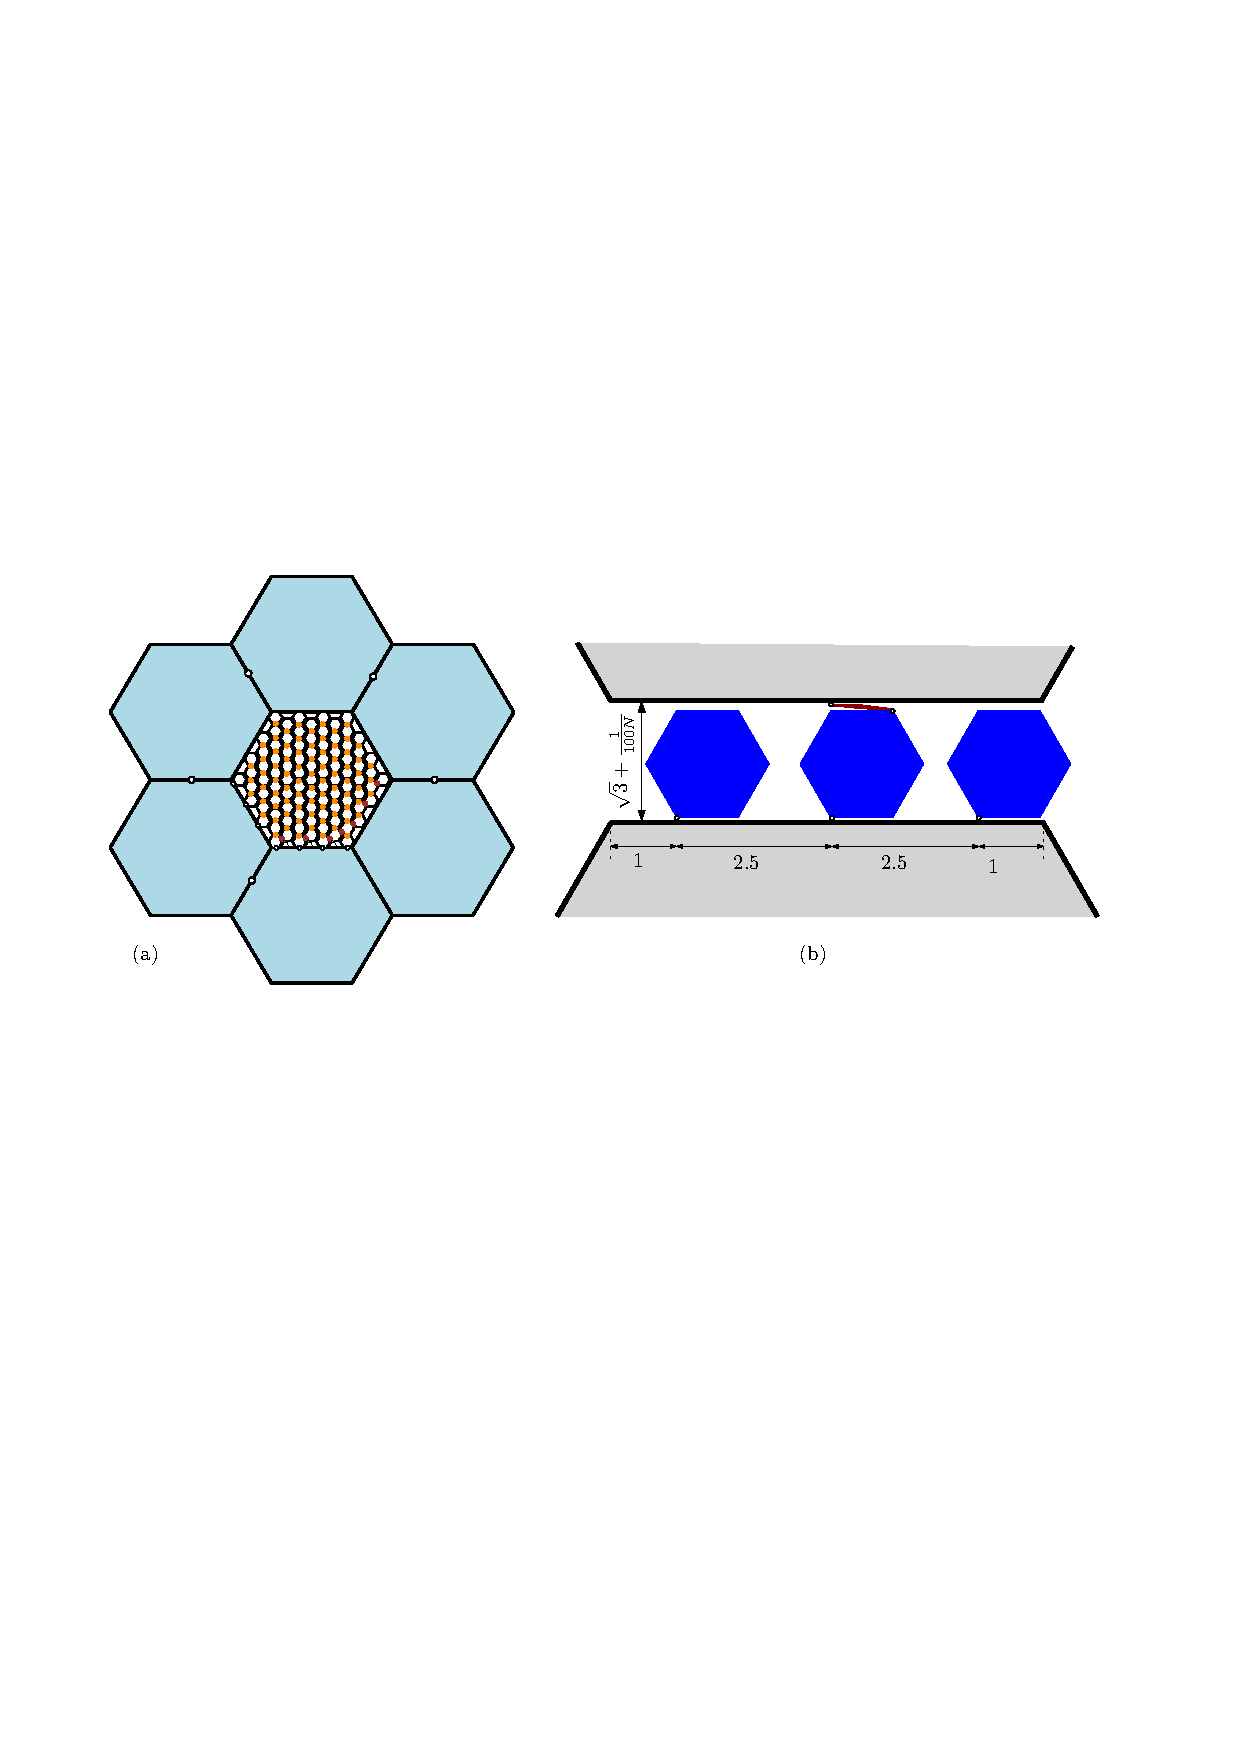
\includegraphics[width=0.95\columnwidth]{graphics/fig-frame-hex}
	\caption{(a) A frame (built of 6 hinged regular hexagons) encloses a hexagonal tiling, and
    vertical paths connect all obstacle hexagons to the frame.
    (b) A corridor is widened to $\sqrt{3}+1/N^2$. A connection between
    two adjacent obstacle hexagons is established via a skinny rhombus.}
	\label{fig:frame}
\end{figure}
We obtain a simply connected polygonal linkage. 
We now allow the obstacle hexagons to move freely, and call their original fixed position \emph{canonical}. 
\noindent (3) We may assume without loss of generality that the frame is at its original position. 
It is enough to show that the obstacle hexagons are still confined to an $1/N$-neighborhood of their canonical position, then it
follows that the polygonal linkage is realizable if and only if $\Phi$ is satisfiable.

\begin{lem}\label{lem:aux}
For every instance $\Phi$ of P3SAT, the above polygonal linkage with flexible and obstacle polygons has the following properties: (1) it has polynomial size; (2) the hinge graph of the modified auxilary construction is a tree;
(3) it admits a realization such that the obstacle polygons remain fixed if and only if $\Phi$ is satisfiable.
\end{lem}







%To show that the hinge graph is a forest, we construct a simply connected polygonal linkage $(\PP,H)$ that has a realization with fixed orientation if and only if $\Phi$ is satisfiable.
























































































































































% \subsection{Functionality of the Auxilary Construction and Gadgets}
% %Prove Observation 1
% %Prove Observation 2
% %Prove Observation 3
% %Prove Lemma 2
% %Prove Lemma 3 - same as lemma 2 but with tree
% %
% We have described the auxiliary construction.  

% Since the height of the corridor is $\sqrt{3}$, each hexagon has exactly two possible realizations: it can lie either \emph{left} or \emph{right} of the hinge in a horizontal corridor. 
% For simplicity, we use the same notation (R and L) in nonhorizontal corridors, too. 
% Hence, the \emph{state} of each flexible hexagon in a realization is either L or R. The following observation describes the key mechanism of a corridor.

% \begin{observation}\label{obs:corridor}
% \begin{itemize}
% \item[(1)] If the leftmost hexagon is in state R, then all $t$ hexagons are in state R, and the rightmost hexagon enters the junction on the right of the corridor.
% \item[(2)] Similarly, if the rightmost hexagon is in state L, then all $t$ hexagons are in state L, and the leftmost hexagon enters the junction on the left of the corridor.
% \end{itemize}
% \end{observation}
% The proof of Obesrvation \ref{obs:junction} is as follows:
% \begin{proof}\label{proof:junction}
% PROOF GOES HERE
% \end{proof}

% Prove that all flexagons around a variable gadget are either clockwise or counterclockwise


% Prove that 

% The following lemma summarizes our result about the auxiliary construction.
% \begin{lem}\label{lem:aux}
% For every instance $\Phi$ of P3SAT, the above polygonal linkage with flexible and obstacle polygons has the following properties: (1) it has polynomial size; (2) its hinge graph is a forest;
% (3) it admits a realization such that the obstacle polygons remain fixed if and only if $\Phi$ is satisfiable.
% \end{lem}
% \begin{proof}

% Suppose we have an instance $\Phi$ of P3SAT with $m$ variables and $n$ clauses with a corresponding associated graph $A(\Phi)=(V,E)$ and it is satisfiable.  
% We need to show the following three properties about its corresponding auxilliary construnction: it has polynomial size, its hinge graph is a forest, and it admits a realization such that the obstacle polygons remain fixed.

% \noindent (1) We can bound the number of obstacle hexagons to represent a variable gadget by $2 D$, where $D = \lr{ \max_{v \in V} \deg (v)}$.  
% The number of clause junctions is $n$.
% To give an upper bound on the number of flexible hexagons in the auxiliary construction, we have to account for the flexible hexagons in the transmitter gadgets, the extra hexagons found in junctions, and the flexible hexagons around the variable gadgets.

% Recall that that the number of flexible hexagons in a corridor are $ t = 2N(m,n)^3 + 1 $ where $N(m,n)$ is a polynomial. 
% Recall that the drawing of $A(\Phi)$ have edges drawn in vertically and horizontally and can join at some ``elbow''.  
% The distance can be measured in the $\ell_1$ norm.
% Similarly in the honeycomb construction, the flexable hexagons zig-zig vertically and horizontally through out honeycomb.  
% The number of corridors about an obstacle hexagon is $6$.
% To give a generous upper bound on the number of flexible hexagons in a transmitter gadget, is $6 \cdot t \cdot \ell_1\lr{v_i,C_j}$, assuming each obstacle hexagon is of unit height.

% The number of junctions in the auxiliary construction is the number of junctions to form all variable gadgets, transmitter gadgets, and clause gadgets. 
% We know there are at most $2 \cdot D$ obstacle hexagons to form each variable gadget and $6$ junctions for each obstacle hexagon.  
% Therefore an upper bound for the number of flexible hexagons around variable gadgets is $m \cdot 6 \cdot t \cdot 2 \cdot D$.
% The upper bound for the number of junctions in a transmitter gadget is $6 \ell_1 \lr{v_i, C_j}$.  
% Thus, the upper bound of all junctions in all transmitter gadgets is $$6 \cdot \sum_{\left\lbrace v_i, C_j \right\rbrace \in E} \ell_1 \lr{v_i, C_j}.$$
% The upper bound on the total number of flexible hexagons is
% $$m \cdot 6 \cdot t \cdot 2 \cdot D + 6 \cdot \sum_{\left\lbrace v_i, C_j \right\rbrace \in E} \ell_1 \lr{v_i, C_j}.$$

% \noindent (2) Recall that a forest is a disjoint union of trees. 
% By construction, each flexible hexagon is hinged to exactly one obstacle hexagon.  
% There are no hinges between obstacle hexagons.
% Consequently, each component of the hinge graph is a star, where the center corresponds to an obstacle hexagon and the leafs corresponds to the flexable hexagons attached to it.

% \noindent (3) 

% To show that the hinge graph is a forest, we construct a simply connected polygonal linkage $(\PP,H)$ that has a realization with fixed orientation if and only if $\Phi$ is satisfiable.
% We modify the auxiliary construction allowing all polygons to move freely, and by adding extra polygons and hinges so that the hinge graph becomes a \emph{tree}, and the size of the construction remains polynomial. 
% Recall that our auxiliary construction is based on a polynomial section of the hexagonal grid, using obstacle hexagons of side lengths $(5t-1)/2$, unit hexagons (of side length 1), and small hexagons of side length $\frac{1}{3}$. 
% We modify it in 3 steps as follows.

% \begin{enumerate}
% \item Move the obstacle hexagons apart such that the width of each corridor increases from $\sqrt{3}$ to $\sqrt{3}+1/(100N)$.
% \item Replace the unit segment in each the clause gadget by a skinny rhombus of diameter $1.1$ and width $1/(200N)$.
% \item Consider a large (polynomial-size) regular hexagon $R$ that contains all gadgets in our construction, and enclose $R$ by a \emph{frame} of 6 congruent regular hexagons, as shown in Fig.~\ref{fig:frame}(a), hinged together in a path.
% \item Connect the frame and the obstacles in $R$ into a simply connected polygonal linkage: In each obstacle hexagon, the bottom or bottom-left side is adjacent to the frame or to a corridor. Introduce a hinge at the midpoint of one such side in each obstacle hexagon. If this side is adjacent to the frame, then attach the hinge to the frame. Otherwise, the hinge is attached to a new \emph{connector} polygon: a skinny rhombus of diameter 1 and width $1/(200N)$. The far corner of each rhombus is hinged to the unit hexagon in the middle of the corridor at shown in Fig.~\ref{fig:frame}(b).
% \end{enumerate}

% \begin{figure}[htbp]
% 	\centering
% 	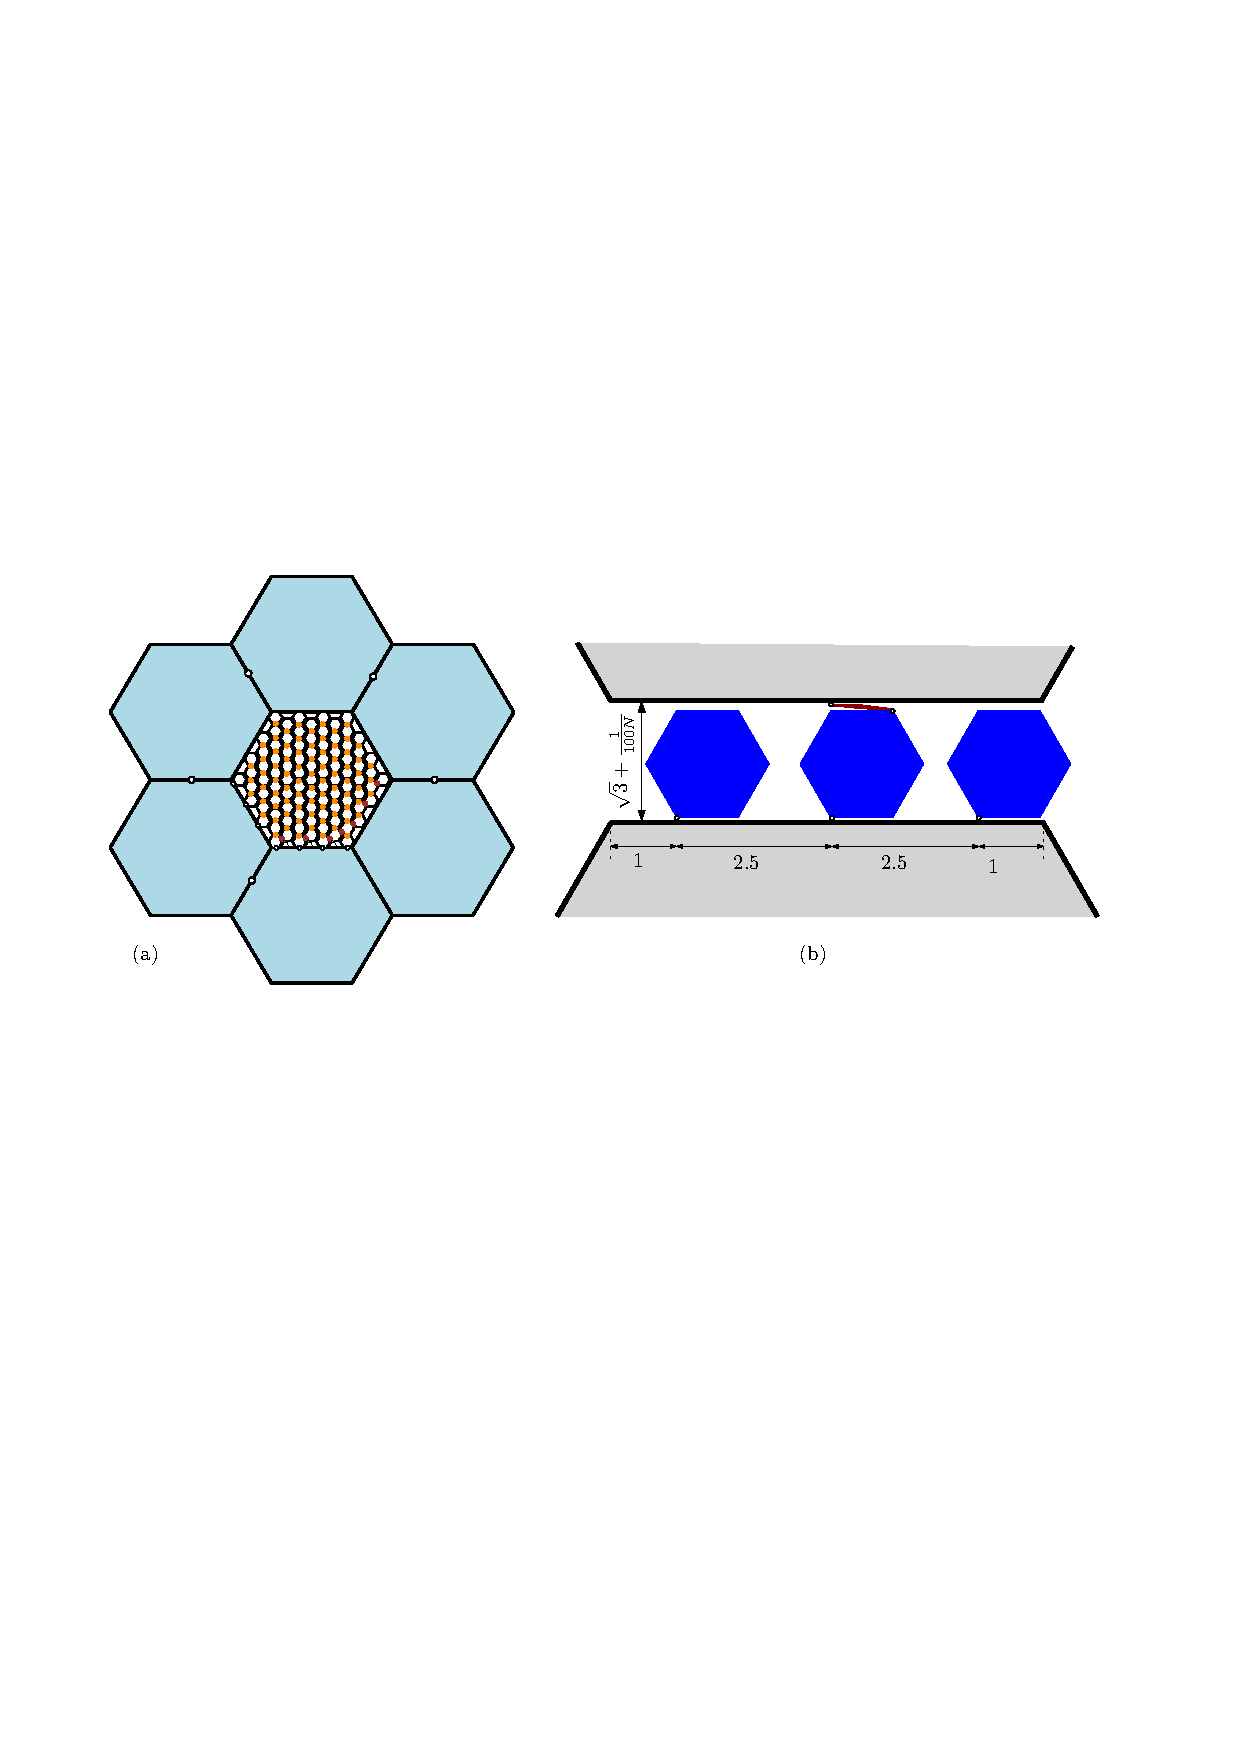
\includegraphics[width=0.95\columnwidth]{graphics/fig-frame-hex}
% 	\caption{(a) A frame (built of 6 hinged regular hexagons) encloses a hexagonal tiling, and
%     vertical paths connect all obstacle hexagons to the frame.
%     (b) A corridor is widened to $\sqrt{3}+1/N^2$. A connection between
%     two adjacent obstacle hexagons is established via a skinny rhombus.}
% 	\label{fig:frame}
% \end{figure}
% We obtain a simply connected polygonal linkage. 
% We now allow the obstacle hexagons to move freely, and call their original fixed position \emph{canonical}. 
% \noindent (3) We may assume without loss of generality that the frame is at its original position. 
% It is enough to show that the obstacle hexagons are still confined to an $1/N$-neighborhood of their canonical position, then it
% follows that the polygonal linkage is realizable if and only if $\Phi$ is satisfiable.






% %Let $\Phi$ be an instance of P3SAT (i.e., a Boolean formula $\Phi$ in 3-CNF with $n$ variables, $m$ clauses, and a planar graph $A(\Phi)$).



% \end{proof}
% The modification of the auxiliary construction is a tree.  
% Satisfiability is an NP-hard problem \cite{cook1971complexity}.
% Thus, we prove Theorem \ref{thm:hinge2}

% The obstacle hexagons in the bottom and bottom-left rows are hinged directly to the frame,
% and so they are locked in their canonical position. Consider two obstacle hexagons on opposite
% sides of a corridor with connector. The distance between the midpoints of the opposite sides of
% the corridor is at least $\sqrt{3}$ (due to the unit hexagons in the corridor) and at most
% $1+\sqrt{3}$ (due to the connector polygon). The length of the corridor is much larger,
% $(5t-1)/2=5N^3+2$, so the orientations of the two adjacent obstacles differ by at most $1/2N^3$.
% Consequently, the orientation of \emph{any} obstacle differs from canonical by at most $1/2N^2$.
% Due to the unit hexagons within the horizontal corridors, the length of any vertical segment between
% the opposite sides of a horizontal corridor is at least $1-1/N^2$. The vertical distance between the
% bottom and top sides of the frame gives an upper bound of  $2N/(100N^2)=1/(50N)$ for the sum of these
% vertical distances. We conclude that the $y$-coordinates of the obstacles are within $1/(10N)$
% of the canonical position. Due to the connector polygons, the $x$-coordinates of
% two adjacent obstacles differ by either less than the vertical offset or by about
% one unit. However, the horizontal distance between the left and right frames prevent
% a shift of this magnitude. So the $x$-coordinates of the obstacle hexagons are also
% within $1/N$ of the canonical position.

